\documentclass[tikz,border=2pt]{standalone}
\usepackage{amsmath,amssymb}
\usepackage{tikz}
\usetikzlibrary{arrows.meta,positioning}

\begin{document}
% Transportation problem: two plants (supplies 30, 20) ship to three centres (demands
% 15, 20, 15) at unit costs on the edges; the optimal shipments (green) cost 125.
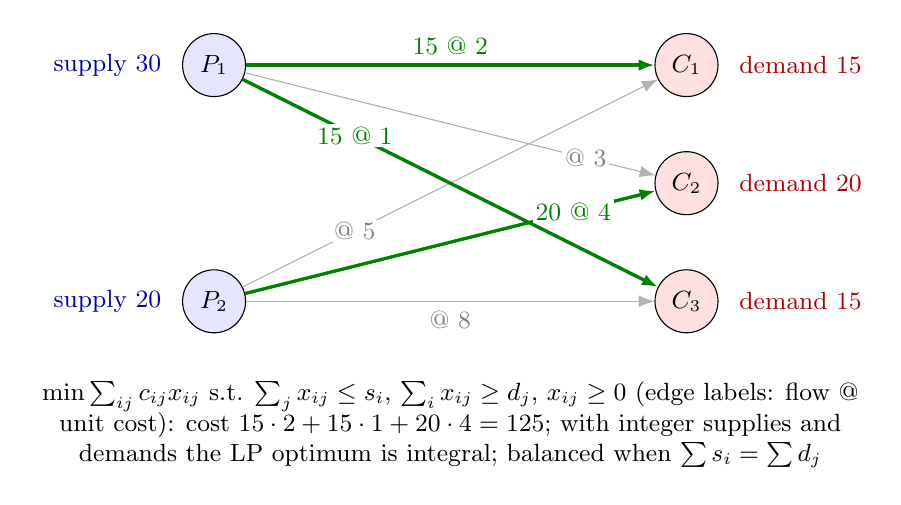
\begin{tikzpicture}[every node/.style={font=\small}, >={Latex[length=2mm]}, v/.style={draw, circle, fill=blue!10, minimum size=8mm, inner sep=0pt}, w/.style={draw, circle, fill=red!12, minimum size=8mm, inner sep=0pt}, el/.style={font=\small, fill=white, inner sep=1pt}]
	\node[v] (p1) at (0,1.5) {$P_1$}; \node[v] (p2) at (0,-1.5) {$P_2$};
	\node[blue!70!black, font=\small, left=4pt of p1] {supply $30$};
	\node[blue!70!black, font=\small, left=4pt of p2] {supply $20$};
	\foreach \j in {1,2,3} {\node[w] (c\j) at (6,{3-1.5*\j}) {$C_\j$};}
	\node[red!70!black, font=\small, right=4pt of c1] {demand $15$};
	\node[red!70!black, font=\small, right=4pt of c2] {demand $20$};
	\node[red!70!black, font=\small, right=4pt of c3] {demand $15$};
	\draw[->, gray!60] (p1) -- (c2) node[pos=0.83, el, text=gray] {@ $3$};
	\draw[->, gray!60] (p2) -- (c1) node[pos=0.27, el, text=gray] {@ $5$};
	\draw[->, gray!60] (p2) -- (c3) node[pos=0.5, below, font=\small, gray] {@ $8$};
	\draw[->, green!50!black, very thick] (p1) -- (c1) node[pos=0.5, above, font=\small] {$15$ @ $2$};
	\draw[->, green!50!black, very thick] (p1) -- (c3) node[pos=0.27, el] {$15$ @ $1$};
	\draw[->, green!50!black, very thick] (p2) -- (c2) node[pos=0.8, el] {$20$ @ $4$};
	\node[anchor=north, align=flush center, text width=10.5cm] at (3.0,-2.4) {$\min\sum_{ij}c_{ij}x_{ij}$ s.t. $\sum_jx_{ij}\le s_i$, $\sum_ix_{ij}\ge d_j$, $x_{ij}\ge0$ (edge labels: flow @ unit cost): cost $15\cdot2+15\cdot1+20\cdot4=125$; with integer supplies and demands the LP optimum is integral; balanced when $\sum s_i=\sum d_j$};
\end{tikzpicture}
\end{document}
